\documentclass[12pt]{article}
\usepackage[paperwidth=52cm, paperheight=22cm, margin=0.5cm]{geometry}
\usepackage{tikz}
\usetikzlibrary{positioning, arrows.meta, calc, decorations.pathreplacing}
\pagestyle{empty}

% ============================================================================
% COLORES
% ============================================================================
\definecolor{pastelblue}{RGB}{230, 242, 252}

% ============================================================================
% TIKZ STYLES
% ============================================================================
\tikzset{
  box/.style={
    draw, thick, fill=pastelblue,
    minimum height=1.5cm,
    minimum width=2cm,
    font=\small\sffamily,
    align=center
  },
  ffbox/.style={
    draw, thick, fill=pastelblue,
    minimum width=3.6cm, 
    minimum height=2cm,
    font=\small\sffamily,
    align=center
  },
  signal/.style={-{Stealth[length=2mm]}, thick, black}, 
  wirelabel/.style={font=\tiny\sffamily, text=black, midway, above}
}

% Triangulo de reloj para flip-flops
\newcommand{\clkpin}[1]{
  \draw[thick] ([yshift=-4mm, xshift=0mm]#1.west) -- ++(2.5mm, 2.5mm) -- ++(-2.5mm, 2.5mm);
}

% MUX 2-a-1
\newcommand{\drawmux}[4]{
  \draw[thick, fill=pastelblue] (#1-0.4,#2+0.8) -- (#1+0.4,#2+0.4) -- (#1+0.4,#2-0.4) -- (#1-0.4,#2-0.8) -- cycle;
  \node[font=\tiny\sffamily] at (#1-0.15, #2+0.4) {0};
  \node[font=\tiny\sffamily] at (#1-0.15, #2-0.4) {1};
  \coordinate (#3_in0) at (#1-0.4, #2+0.4);
  \coordinate (#3_in1) at (#1-0.4, #2-0.4);
  \coordinate (#3_in2) at (#1-0.4, #2); 
  \coordinate (#3_out) at (#1+0.4, #2);
  \coordinate (#3_sel) at (#1, #2+0.6);
}

% MUX 3-a-1
\newcommand{\drawmuxthree}[4]{
  \draw[thick, fill=pastelblue] (#1-0.4,#2+1.0) -- (#1+0.4,#2+0.6) -- (#1+0.4,#2-0.6) -- (#1-0.4,#2-1.0) -- cycle;
  \node[font=\tiny\sffamily] at (#1-0.15, #2+0.6) {00};
  \node[font=\tiny\sffamily] at (#1-0.15, #2) {01};
  \node[font=\tiny\sffamily] at (#1-0.15, #2-0.6) {10};
  \coordinate (#3_in0) at (#1-0.4, #2+0.6);
  \coordinate (#3_in1) at (#1-0.4, #2);
  \coordinate (#3_in2) at (#1-0.4, #2-0.6);
  \coordinate (#3_out) at (#1+0.4, #2);
  \coordinate (#3_sel) at (#1, #2+0.8);
}

% Compuerta AND
\newcommand{\drawand}[3]{
  \draw[thick, fill=pastelblue] (#1-0.4, #2+0.4) -- (#1, #2+0.4) arc (90:-90:0.4) -- (#1-0.4, #2-0.4) -- cycle;
  \coordinate (#3_in1) at (#1-0.4, #2+0.2);
  \coordinate (#3_in2) at (#1-0.4, #2-0.2);
  \coordinate (#3_out) at (#1+0.4, #2);
}

% Compuerta OR
\newcommand{\drawor}[3]{
  \draw[thick, fill=pastelblue] (#1-0.4, #2+0.4) .. controls (#1-0.1, #2+0.4) and (#1+0.4, #2+0.1) .. (#1+0.4, #2) .. controls (#1+0.4, #2-0.1) and (#1-0.1, #2-0.4) .. (#1-0.4, #2-0.4) .. controls (#1-0.2, #2-0.1) and (#1-0.2, #2+0.1) .. (#1-0.4, #2+0.4) -- cycle;
  \coordinate (#3_in1) at (#1-0.35, #2+0.2);
  \coordinate (#3_in2) at (#1-0.35, #2-0.2);
  \coordinate (#3_out) at (#1+0.4, #2);
}

% ALU
\newcommand{\drawalu}[3]{
  \draw[thick, fill=pastelblue] 
    (#1-0.8, #2+1.5) -- 
    (#1-0.8, #2+0.3) -- 
    (#1-0.4, #2) -- 
    (#1-0.8, #2-0.3) -- 
    (#1-0.8, #2-1.5) -- 
    (#1+0.8, #2-0.8) -- 
    (#1+0.8, #2+0.8) -- cycle;
  \node[font=\small\sffamily] (#3) at (#1+0.1, #2) {ALU};
  \coordinate (#3_in1) at (#1-0.8, #2+0.8);
  \coordinate (#3_in2) at (#1-0.8, #2-0.8);
  \coordinate (#3_out) at (#1+0.8, #2);
  \coordinate (#3_zero) at (#1+0.8, #2+0.5);
  \coordinate (#3_sel) at (#1, #2+1.1);
}

% Adder
\newcommand{\drawadder}[3]{
  \draw[thick, fill=pastelblue] 
    (#1-0.6, #2+1.0) -- 
    (#1-0.6, #2+0.2) -- 
    (#1-0.3, #2) -- 
    (#1-0.6, #2-0.2) -- 
    (#1-0.6, #2-1.0) -- 
    (#1+0.6, #2-0.5) -- 
    (#1+0.6, #2+0.5) -- cycle;
  \node[font=\small\sffamily] (#3) at (#1+0.1, #2) {$+$};
  \coordinate (#3_in1) at (#1-0.6, #2+0.5);
  \coordinate (#3_in2) at (#1-0.6, #2-0.5);
  \coordinate (#3_out) at (#1+0.6, #2);
}

% Extend
\newcommand{\drawextend}[3]{
  \draw[thick, fill=pastelblue] 
    (#1-1.2, #2+0.3) -- 
    (#1+1.2, #2+0.6) -- 
    (#1+1.2, #2-0.6) -- 
    (#1-1.2, #2-0.3) -- cycle;
  \node[font=\small\sffamily] (#3) at (#1, #2) {Extend};
  \coordinate (#3_in) at (#1-1.2, #2);
  \coordinate (#3_out) at (#1+1.2, #2);
}

% ============================================================================
% INICIO DEL DOCUMENTO
% ============================================================================
\begin{document}
\centering
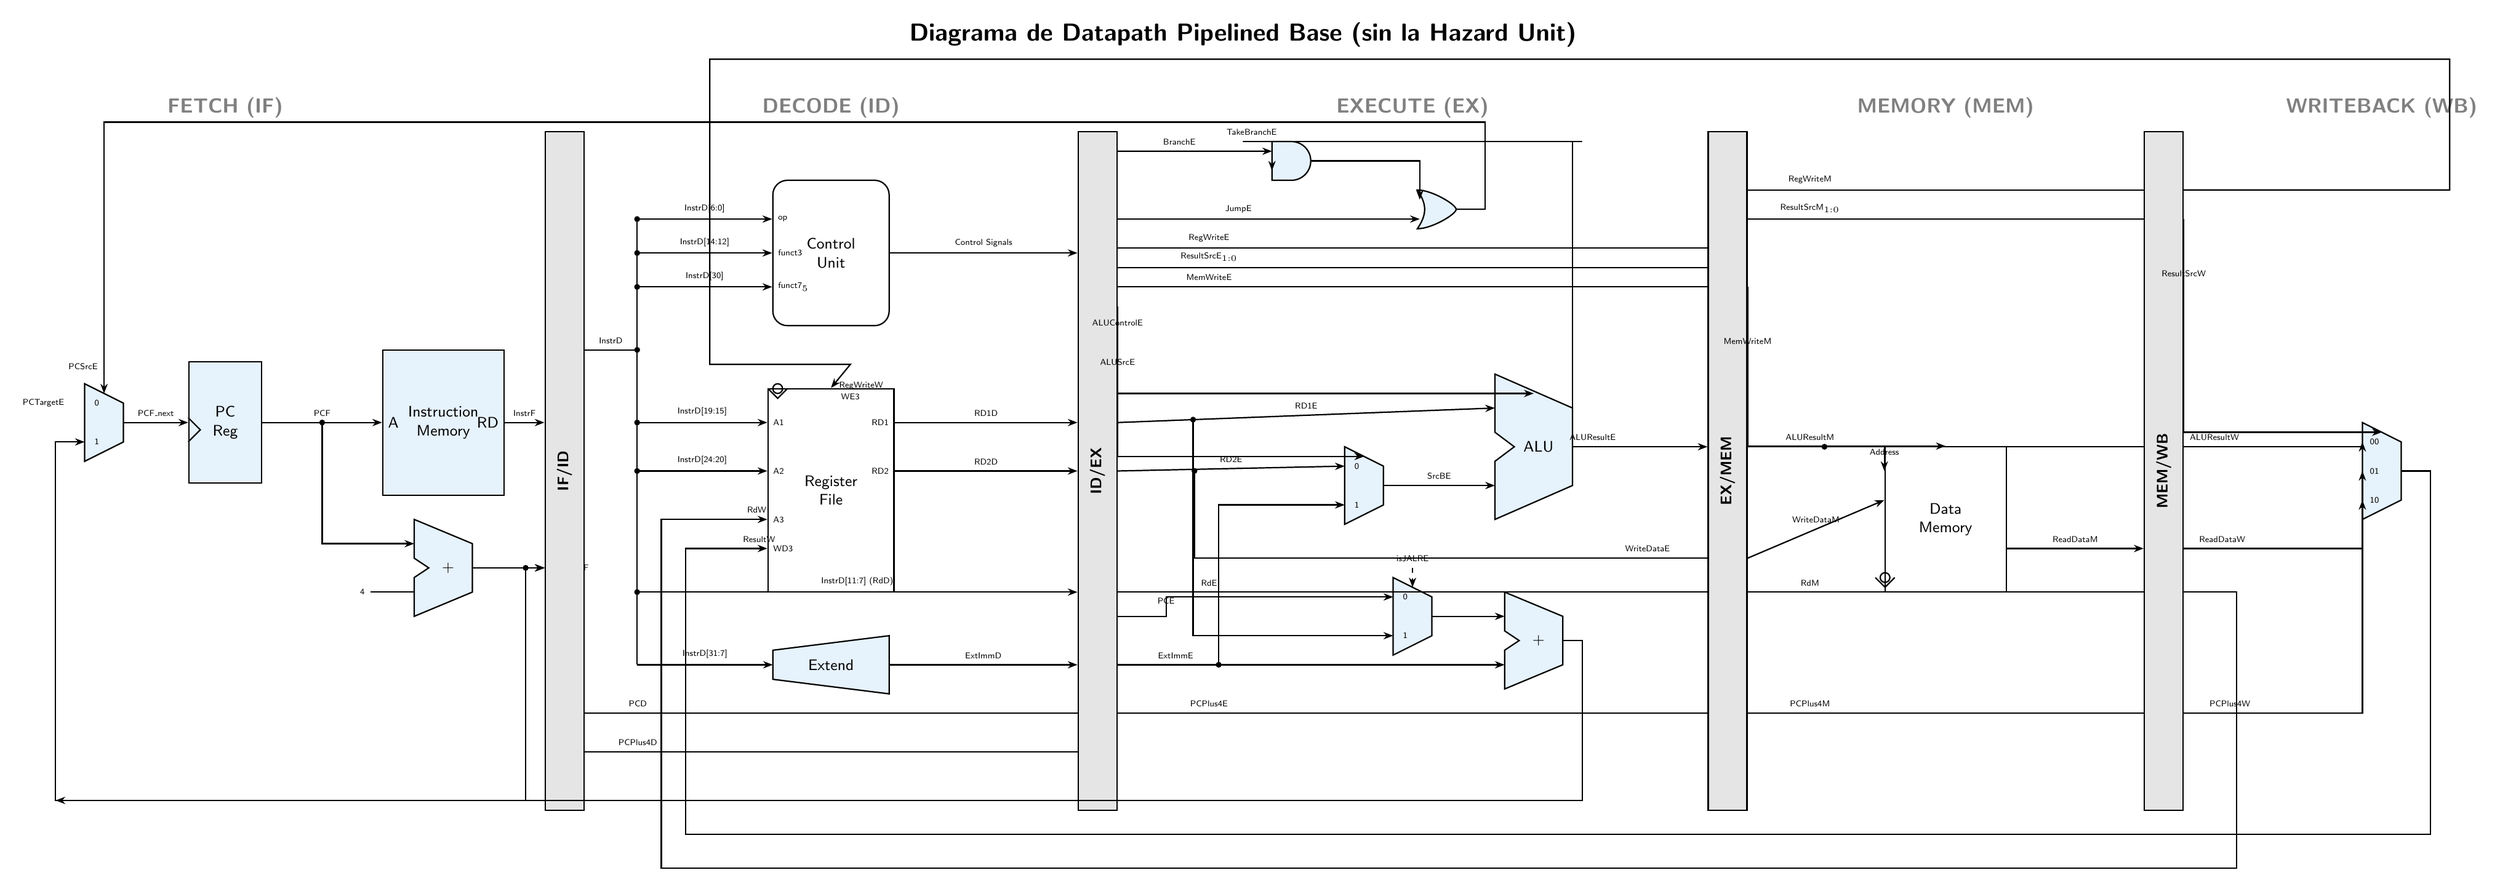
\begin{tikzpicture}[
  x=1cm, y=1cm,
  signal/.style={-{Stealth[length=2mm]}, thick, black},
  lbl/.style={font=\tiny\sffamily, text=black},
  lblcenter/.style={font=\small\sffamily, align=center},
]

  % Titulo
  \node[font=\Large\sffamily\bfseries] at (20, 9) {Diagrama de Datapath Pipelined Base (sin la Hazard Unit)};

  % ============================================================================
  % ETAPA 1: FETCH (IF)
  % ============================================================================
  \node[font=\large\sffamily\bfseries, text=gray] at (-1, 7.5) {FETCH (IF)};

  % Mux PC
  \drawmux{-3.5}{1.0}{pcmux}{}
  \node[lbl, left] at (-4.2, 1.4) {PCTargetE};

  % Registro PC
  \node[box, minimum height=2.5cm, minimum width=1.5cm] (pcreg) at (-1.0, 1.0) {};
  \node[lblcenter] at (-1.0, 1.0) {PC\\Reg};
  \clkpin{pcreg}

  % Memoria de Instrucciones
  \node[box, minimum height=3.0cm, minimum width=2.5cm] (imem) at (3.5, 1.0) {};
  \node[lblcenter] at (3.5, 1.0) {Instruction\\Memory};
  \node[font=\small\sffamily, right] at (imem.west |- {0,1}) {A};
  \node[font=\small\sffamily, left] at (imem.east |- {0,1}) {RD};

  % Adder (+4)
  \drawadder{3.5}{-2.0}{add4}

  % Conexiones Fetch
  \draw[signal] (pcmux_out) -- (pcreg.west) node[midway, above, lbl] {PCF\_next};
  \draw[signal] (pcreg.east) -- (imem.west |- {0,1}) node[midway, above, lbl] {PCF};
  \draw[fill=black] (1.0, 1.0) circle (1.5pt);
  \draw[signal] (1.0, 1.0) |- (add4_in1);
  \draw[thick] (2.0, -2.5) -- (add4_in2);
  \node[left, lbl] at (2.0, -2.5) {4};
  
  % Feedback PCPlus4F
  \draw[signal] (add4_out) -- ++(1.5, 0) node[right, lbl] {PCPlus4F};
  \draw[fill=black] (5.2, -2.0) circle (1.5pt);
  \draw[signal] (5.2, -2.0) |- (5.2, -6.8) -- (-4.5, -6.8) |- (-4.5, 0.6) -- (pcmux_in1);

  % ============================================================================
  % REGISTRO PIPELINE IF/ID
  % ============================================================================
  \node[draw, fill=gray!20, thick, minimum width=0.8cm, minimum height=14cm, font=\small\sffamily\bfseries] (ifid) at (6.0, 0) {\rotatebox{90}{IF/ID}};
  \draw[signal] (imem.east |- {0,1}) -- (ifid.west |- {0,1}) node[midway, above, lbl] {InstrF};
  \draw[signal] (5.2, -2.0) |- (ifid.west |- {0, -2.0});

  % ============================================================================
  % ETAPA 2: DECODE (ID)
  % ============================================================================
  \node[font=\large\sffamily\bfseries, text=gray] at (11.5, 7.5) {DECODE (ID)};

  % Control Unit
  \node[draw, thick, fill=white, rounded corners=3mm, minimum height=3.0cm, minimum width=2.4cm, font=\small\sffamily, align=center] (ctrl) at (11.5, 4.5) {Control\\Unit};
  \node[font=\tiny\sffamily, right] at (ctrl.west |- {0,5.2}) {op};
  \node[font=\tiny\sffamily, right] at (ctrl.west |- {0,4.5}) {funct3};
  \node[font=\tiny\sffamily, right] at (ctrl.west |- {0,3.8}) {funct7$_5$};

  % Register File
  \node[draw, thick, fill=white, minimum height=4.2cm, minimum width=2.6cm] (regfile) at (11.5, -0.4) {};
  \node[lblcenter] at (11.5, -0.4) {Register\\File};
  \node[font=\tiny\sffamily, right] at (regfile.west |- {0, 1.0}) {A1};
  \node[font=\tiny\sffamily, right] at (regfile.west |- {0, 0.0}) {A2};
  \node[font=\tiny\sffamily, right] at (regfile.west |- {0, -1.0}) {A3};
  \node[font=\tiny\sffamily, right] at (regfile.west |- {0, -1.6}) {WD3};
  \node[font=\tiny\sffamily, left]  at (regfile.east |- {0, 1.0}) {RD1};
  \node[font=\tiny\sffamily, left]  at (regfile.east |- {0, 0.0}) {RD2};
  \node[font=\tiny\sffamily, below] at (regfile.north -| {11.9, 0}) {WE3};
  \draw[thick] (10.4, 1.7) circle (1mm);
  \draw[thick] (10.2, 1.7) -- ++(2mm, -2mm) -- ++(2mm, 2mm); % clk pin

  % Extend Unit
  \drawextend{11.5}{-4.0}{ext}

  % Conexiones Decode
  \draw[thick, black] (ifid.east |- {0,2.5}) -- (7.5, 2.5) node[midway, above, lbl] {InstrD};
  \draw[thick, black] (7.5, 5.2) -- (7.5, -4.0);
  \draw[fill=black] (7.5, 2.5) circle (1.5pt);

  \draw[signal] (7.5, 5.2) -- (ctrl.west |- {0,5.2}) node[lbl, midway, above] {InstrD[6:0]};
  \draw[fill=black] (7.5, 5.2) circle (1.5pt);
  \draw[signal] (7.5, 4.5) -- (ctrl.west |- {0,4.5}) node[lbl, midway, above] {InstrD[14:12]};
  \draw[fill=black] (7.5, 4.5) circle (1.5pt);
  \draw[signal] (7.5, 3.8) -- (ctrl.west |- {0,3.8}) node[lbl, midway, above] {InstrD[30]};
  \draw[fill=black] (7.5, 3.8) circle (1.5pt);

  \draw[signal] (7.5, 1.0) -- (regfile.west |- {0,1.0}) node[lbl, midway, above] {InstrD[19:15]};
  \draw[fill=black] (7.5, 1.0) circle (1.5pt);
  \draw[signal] (7.5, 0.0) -- (regfile.west |- {0,0.0}) node[lbl, midway, above] {InstrD[24:20]};
  \draw[fill=black] (7.5, 0.0) circle (1.5pt);

  \draw[signal] (7.5, -4.0) -- (ext_in) node[lbl, midway, above] {InstrD[31:7]};

  % PCD and PCPlus4D passing straight through
  \draw[signal] (ifid.east |- {0,-5.0}) -- ++(11, 0) node[lbl, pos=0.1, above] {PCD};
  \draw[signal] (ifid.east |- {0,-5.8}) -- ++(11, 0) node[lbl, pos=0.1, above] {PCPlus4D};

  % ============================================================================
  % REGISTRO PIPELINE ID/EX
  % ============================================================================
  \node[draw, fill=gray!20, thick, minimum width=0.8cm, minimum height=14cm, font=\small\sffamily\bfseries] (idex) at (17.0, 0) {\rotatebox{90}{ID/EX}};
  
  \draw[signal] (ctrl.east |- {0,4.5}) -- (idex.west |- {0,4.5}) node[lbl, midway, above] {Control Signals};
  \draw[signal] (regfile.east |- {0,1.0}) -- (idex.west |- {0,1.0}) node[lbl, midway, above] {RD1D};
  \draw[signal] (regfile.east |- {0,0.0}) -- (idex.west |- {0,0.0}) node[lbl, midway, above] {RD2D};
  \draw[signal] (ext_out) -- (idex.west |- ext_out) node[lbl, midway, above] {ExtImmD};
  
  % RdD (InstrD[11:7])
  \draw[signal] (7.5, -2.5) -- (idex.west |- {0,-2.5}) node[lbl, midway, above] {InstrD[11:7] (RdD)};
  \draw[fill=black] (7.5, -2.5) circle (1.5pt);

  % ============================================================================
  % ETAPA 3: EXECUTE (EX)
  % ============================================================================
  \node[font=\large\sffamily\bfseries, text=gray] at (23.5, 7.5) {EXECUTE (EX)};

  % Mux ALUSrcE (Mux S)
  \drawmux{22.5}{-0.3}{muxS}{}

  % ALU
  \drawalu{26.0}{0.5}{myalu}

  % Target Address Adder
  \drawadder{26.0}{-3.5}{addT}

  % Branch/Jump decision gates
  \drawand{21.0}{6.4}{and_gate}
  \drawor{24.0}{5.4}{or_gate}

  % Conexiones Execute
  \draw[signal] (idex.east |- {0,1.0}) -- (myalu_in1) node[lbl, midway, above] {RD1E};
  \draw[signal] (idex.east |- {0,0.0}) -- (muxS_in0) node[lbl, midway, above] {RD2E};
  
  % Tap to WriteDataE (passes directly to EX/MEM)
  \draw[fill=black] (19.0, 0.0) circle (1.5pt);
  \draw[signal] (19.0, 0.0) |- (19.0, -1.8) -- (30.0, -1.8) node[lbl, pos=0.85, above] {WriteDataE};

  \draw[signal] (idex.east |- {0,-4.0}) -- (addT_in2) node[lbl, pos=0.15, above] {ExtImmE};
  \draw[fill=black] (19.5, -4.0) circle (1.5pt);
  \draw[signal] (19.5, -4.0) |- (muxS_in1);

  \draw[signal] (muxS_out) -- (myalu_in2) node[lbl, midway, above] {SrcBE};

  % Mux PC Target Base for JALR
  \drawmux{23.5}{-3.0}{jalrmux}{}
  \draw[signal] (idex.east |- {0,-3.0}) -- ++(1.0, 0) |- (jalrmux_in0) node[lbl, pos=0.15, above] {PCE};
  \path (idex.east |- {0,1.0}) -- (myalu_in1) coordinate[pos=0.2] (tap_rd1);
  \draw[fill=black] (tap_rd1) circle (1.5pt);
  \draw[signal] (tap_rd1) |- (jalrmux_in1);
  \draw[signal] (jalrmux_out) -- (addT_in1);
  \draw[signal, dashed] (23.5, -2.0) node[above, lbl] {isJALRE} -- (jalrmux_sel);

  % Control signals to execution blocks
  \draw[signal] (idex.east |- {0, 3.4}) |- (myalu_sel) node[lbl, pos=0.15, above] {ALUControlE};
  \draw[signal] (idex.east |- {0, 2.8}) |- (muxS_sel) node[lbl, pos=0.15, above] {ALUSrcE};

  % Control signals passing straight through EX stage
  \draw[signal] (idex.east |- {0, 4.6}) -- (30, 4.6) node[lbl, pos=0.15, above] {RegWriteE};
  \draw[signal] (idex.east |- {0, 4.2}) -- (30, 4.2) node[lbl, pos=0.15, above] {ResultSrcE$_{1:0}$};
  \draw[signal] (idex.east |- {0, 3.8}) -- (30, 3.8) node[lbl, pos=0.15, above] {MemWriteE};

  % Branch Logic
  \draw[signal] (idex.east |- {0, 6.6}) -- (and_gate_in1) node[lbl, pos=0.4, above] {BranchE};
  \draw[signal] (idex.east |- {0, 5.2}) -- (or_gate_in2) node[lbl, pos=0.4, above] {JumpE};
  \draw[signal] (and_gate_out) -| (or_gate_in1);
  \draw[signal] (myalu_zero) |- (27.0, 6.8) -- (20.0, 6.8) -| (and_gate_in2) node[lbl, pos=0.15, above] {TakeBranchE};

  % Feedback paths from EX
  % PCSrcE feedback
  \draw[signal] (or_gate_out) -- (25.0, 5.4) |- (25.0, 7.2) -- (-3.5, 7.2) -- (pcmux_sel) node[lbl, pos=0.9, left] {PCSrcE};
  % PCTargetE feedback
  \draw[signal] (addT_out) -- (27.0, -3.5) |- (27.0, -6.8) -- (-4.5, -6.8);

  % Other signals passing straight through
  \draw[signal] (idex.east |- {0, -2.5}) -- (30, -2.5) node[lbl, pos=0.15, above] {RdE};
  \draw[signal] (idex.east |- {0, -5.0}) -- (30, -5.0) node[lbl, pos=0.15, above] {PCPlus4E};

  % ============================================================================
  % REGISTRO PIPELINE EX/MEM
  % ============================================================================
  \node[draw, fill=gray!20, thick, minimum width=0.8cm, minimum height=14cm, font=\small\sffamily\bfseries] (exmem) at (30.0, 0) {\rotatebox{90}{EX/MEM}};
  
  \draw[signal] (myalu_out) -- (exmem.west |- myalu_out) node[lbl, pos=0.15, above] {ALUResultE};

  % ============================================================================
  % ETAPA 4: MEMORY (MEM)
  % ============================================================================
  \node[font=\large\sffamily\bfseries, text=gray] at (34.5, 7.5) {MEMORY (MEM)};

  % Data Memory
  \node[draw, thick, fill=white, minimum height=3.0cm, minimum width=2.5cm, font=\small\sffamily, align=center] (dmem) at (34.5, -1.0) {Data\\Memory};
  \draw[thick] (33.25, -2.2) circle (1mm);
  \draw[thick] (33.05, -2.2) -- ++(2mm, -2mm) -- ++(2mm, 2mm); % clk pin

  % Conexiones Memory
  \draw[signal] (exmem.east |- {0, 0.5}) -- (39, 0.5) node[lbl, pos=0.15, above] {ALUResultM};
  \draw[fill=black] (32.0, 0.5) circle (1.5pt);
  \draw[signal] (32.0, 0.5) -| (dmem.west |- {0, 0.0}) node[lbl, pos=0.8, above] {Address};

  \draw[signal] (exmem.east |- {0, -1.8}) -- (dmem.west |- {0,-0.6}) node[lbl, midway, above] {WriteDataM};
  \draw[signal] (exmem.east |- {0, 3.8}) |- (dmem.north) node[lbl, pos=0.2, above] {MemWriteM};

  % Control signals passing straight through
  \draw[signal] (exmem.east |- {0, 5.8}) -- (39, 5.8) node[lbl, pos=0.15, above] {RegWriteM};
  \draw[signal] (exmem.east |- {0, 5.2}) -- (39, 5.2) node[lbl, pos=0.15, above] {ResultSrcM$_{1:0}$};

  % Other signals passing straight through
  \draw[signal] (exmem.east |- {0, -2.5}) -- (39, -2.5) node[lbl, pos=0.15, above] {RdM};
  \draw[signal] (exmem.east |- {0, -5.0}) -- (39, -5.0) node[lbl, pos=0.15, above] {PCPlus4M};

  % ============================================================================
  % REGISTRO PIPELINE MEM/WB
  % ============================================================================
  \node[draw, fill=gray!20, thick, minimum width=0.8cm, minimum height=14cm, font=\small\sffamily\bfseries] (memwb) at (39.0, 0) {\rotatebox{90}{MEM/WB}};
  
  \draw[signal] (dmem.east |- {0, -1.6}) -- (memwb.west |- {0,-1.6}) node[lbl, midway, above] {ReadDataM};

  % ============================================================================
  % ETAPA 5: WRITEBACK (WB)
  % ============================================================================
  \node[font=\large\sffamily\bfseries, text=gray] at (43.5, 7.5) {WRITEBACK (WB)};

  % Result Mux
  \drawmuxthree{43.5}{0.0}{muxR}{}

  % Conexiones Writeback
  \draw[signal] (memwb.east |- {0, 0.5}) -- (41.0, 0.5) node[lbl, pos=0.4, above] {ALUResultW} -| (muxR_in0);
  \draw[signal] (memwb.east |- {0, -1.6}) -- (41.4, -1.6) node[lbl, pos=0.4, above] {ReadDataW} -| (muxR_in1);
  \draw[signal] (memwb.east |- {0, -5.0}) -- (41.8, -5.0) node[lbl, pos=0.4, above] {PCPlus4W} -| (muxR_in2);

  \draw[signal] (memwb.east |- {0, 5.2}) |- (muxR_sel) node[lbl, pos=0.15, above] {ResultSrcW};

  % Feedback paths back to Decode stage
  % ResultW feedback
  \draw[signal] (muxR_out) -- (44.5, 0.0) |- (44.5, -7.5) -- (8.5, -7.5) |- (8.5, -1.6) -- (regfile.west |- {0,-1.6}) node[lbl, pos=0.9, above] {ResultW};
  
  % RdW feedback
  \draw[signal] (memwb.east |- {0, -2.5}) -- (40.5, -2.5) |- (40.5, -8.2) -- (8.0, -8.2) |- (8.0, -1.0) -- (regfile.west |- {0,-1.0}) node[lbl, pos=0.9, above] {RdW};

  % RegWriteW feedback
  \draw[signal] (memwb.east |- {0, 5.8}) -- (44.9, 5.8) |- (44.9, 8.5) -- (9.0, 8.5) |- (11.9, 2.2) -- (regfile.north) node[lbl, pos=0.9, right] {RegWriteW};

\end{tikzpicture}
\end{document}
